%% Scientific Reports submission -- Springer Nature template (sn-jnl.cls)
%% Compile: pdflatex -> bibtex -> pdflatex x2   (Overleaf: set this file as Main document)
\documentclass[pdflatex,sn-nature]{sn-jnl}   % Nature Portfolio reference style

\usepackage{xcolor}
\usepackage{footmisc}\usepackage{manyfoot}   % required by sn-jnl.cls (missing \RequirePackage in the class)
\usepackage{graphicx}
\usepackage{amsmath,amssymb}
\usepackage{soul}\usepackage{url}      % \hl{} highlights kept from the Word draft -- remove before submission
\usepackage{lineno}
%\linenumbers

\raggedbottom

\begin{document}

\title[Beaver DOC control points]{Beaver engineering creates intense, context-dependent dissolved organic carbon control points in streams}

\author*[1,2]{\fnm{Leonardo} \sur{Capitani}}\email{leocapi07@gmail.com}
\author[3,4]{\fnm{Annegret} \sur{Larsen}}
\author[5]{\fnm{Joshua R.} \sur{Larsen}}
\author[6]{\fnm{Matthew} \sur{Dennis}}
\author[4,5]{\fnm{Lukas} \sur{Hallberg}}
\author[1,2]{\fnm{Valentin} \sur{Moser}}
\author[7]{\fnm{Christof} \sur{Angst}}
\author[8]{\fnm{Silvan} \sur{Minnig}}
\author[9]{\fnm{Kaspar} \sur{Berger}}
\author[1]{\fnm{Steffen} \sur{Boch}}
\author[1]{\fnm{Massimiliano} \sur{Zappa}}
\author[2]{\fnm{Francesco} \sur{Pomati}}
\author[1]{\fnm{Anita C.} \sur{Risch}}

\affil[1]{\orgname{WSL - Swiss Federal Institute for Forest, Snow and Landscape Research}, \orgaddress{\city{Birmensdorf}, \country{Switzerland}}}
\affil[2]{\orgdiv{Department of Aquatic Ecology}, \orgname{Eawag - Swiss Federal Institute of Water Science and Technology}, \orgaddress{\city{D\"ubendorf}, \country{Switzerland}}}
\affil[3]{\orgdiv{Soil Geography and Landscape Group}, \orgname{Wageningen University \& Research}, \orgaddress{\country{The Netherlands}}}
\affil[4]{\orgdiv{River Ecosystems Laboratory, Alpine and Polar Environmental Research Center}, \orgname{Ecole Polytechnique F\'ed\'erale de Lausanne}, \orgaddress{\city{Sion}, \country{Switzerland}}}
\affil[5]{\orgdiv{School of Geography, Earth and Environmental Sciences}, \orgname{University of Birmingham}, \orgaddress{\country{UK}}}
\affil[6]{\orgdiv{CIRCLE, Department of Geography, School of Environment and Life Sciences}, \orgname{The University of Manchester}, \orgaddress{\country{UK}}}
\affil[7]{\orgname{Info fauna Nationale Biberfachstelle}, \orgaddress{\city{Neuch\^atel}, \country{Switzerland}}}
\affil[8]{\orgname{umweltbildner.ch}, \orgaddress{\city{Bern}, \country{Switzerland}}}
\affil[9]{\orgdiv{Institute of Geography}, \orgname{University of Bern}, \orgaddress{\country{Switzerland}}}

\abstract{Despite recolonization across Europe, the effects of beavers on freshwater dissolved organic carbon (DOC) concentrations remain understudied. DOC influences microbial activity and energy flow in aquatic food webs. Understanding how and when beaver-engineering alters DOC is therefore critical for predicting its ecosystem consequences. Using a national-scale dataset we quantified the magnitude and drivers of DOC concentration changes associated with beaver-engineering. We found that beaver-engineering exerted negligible influences on DOC in about 76\% of stream samplings, but also promoted DOC source (12--16\%) and sink (9--12\%) responses. Dams modified stream hydrology, which influenced DOC indirectly via changes in primary producer abundance. Relative to the inherited seasonal contrast of upstream DOC, beaver-engineering added DOC equal to 21\% of that contrast in summer (95\% credible interval 11--33\%) and had no net effect in winter, on a footprint of about 0.4\% of the floodplain area. These findings are crucial as they enable stakeholders to predict whether beaver-engineering will increase or decrease DOC concentrations, guiding decisions on where and when beaver presence will affect water quality and ecosystem functioning.}

\keywords{Castor, dam, freshwater, DOC, causal inference, abundance, primary producers, hydrology}

\maketitle

\section{Introduction}

Ecosystem engineers are organisms that modify the physical structure of their environment and thereby control the availability of resources to other organisms \cite{jones1994}. They can profoundly alter ecosystem function without necessarily shifting ecosystem properties in a consistent direction across landscapes: by restructuring habitat, hydrology and resource availability, they create localized control points where biogeochemical processing becomes disproportionately intense \cite{bernhardt2017}, consistent with an increasing appreciation for spatially discrete controls on carbon dynamics within river networks \cite{laudon2026}. Beavers (\emph{Castor fiber} L. and \emph{C. canadensis} Kuhl), whose populations are recovering across Europe and North America with assistance from rewilding and restoration, offer a powerful and increasingly widespread example of such engineering: their dams profoundly influence riparian system hydrology, ecosystems and biogeochemistry \cite{larsen2021,grudzinski2022}.

By damming streams and flooding valley floors, beavers reshape how organic matter and organic carbon move through river corridors. Beaver ponds and the wet meadows around them trap fine sediment and particulate organic carbon, store large amounts of carbon in pond sediments and floodplain soils, and raise water tables in ways that slow the breakdown of that carbon \cite{wohl2012,wohl2013,johnston2014,laurel2019}; when dams are abandoned and ponds drain, this stored carbon can be released again \cite{wohl2013,rees2024}. Beavers also slow the water down, reconnect streams with their floodplains, and open up the tree canopy, which favours the growth of aquatic plants and algae \cite{johnston2017,nummi2018,ray2001}. These changes can enrich the dissolved fraction of organic carbon (dissolved organic carbon, DOC) through the growth and release of compounds by aquatic plants and algae, plant turnover and leaf-litter inputs, and the flooding and leaching of carbon-rich soils \cite{bedzki2010,ciuldiene2020,johnston2017}; but they can equally deplete DOC by slowing the water down long enough for microbes and sunlight to break it down, or by trapping it in sediments and groundwater pathways \cite{nummi2018,ledford2023}. There is therefore no strong theoretical reason to expect beaver ponds to consistently add or remove DOC; indeed, syntheses and reviews find that beaver ponds increase DOC in most, but not all, cases \cite{grudzinski2022,larsen2021}.

DOC itself is key to the carbon (C) cycle and plays an important role in safeguarding freshwater biodiversity and maintaining water quality \cite{allan2021}. It links terrestrial and aquatic carbon pathways and, as a major energy source for microorganisms, provides the substrate for heterotrophic metabolism, influencing microbial respiration, nutrient cycling and overall ecosystem functioning in streams and rivers \cite{meyer1988,battin2023,raza2023}. Elevated DOC can lead to hypoxia or other unfavourable conditions for aquatic life \cite{stanley2012}, and DOC contributes to the formation of disinfection byproducts in drinking water treatment, making its monitoring and management important for human health \cite{leonard2022}. DOC is therefore a critical pathway by which the physical engineering of beavers can be transmitted into food webs and water quality.

Yet, despite the potential impact of beavers on DOC transformations, the effects of beaver-engineering on DOC have been shown to vary widely depending on site-specific factors such as vegetation, soil, hydrology and climate \cite{larsen2021,grudzinski2022}, and DOC dynamics have been studied mostly at individual sites \cite{bedzki2010,ciuldiene2020,ledford2023}. It thus remains unclear whether the inconsistent responses reported among sites represent noise around a common average effect, or whether context-dependent positive and negative responses are themselves a characteristic feature of beaver ecosystem engineering. No large-scale analyses have been available so far to examine how beaver-induced hydrological and biogeochemical modifications influence the timing and magnitude of DOC changes across diverse landscapes. Such an analysis must account for the drivers that control stream DOC independently of beavers: land use within the catchment, the diversity and abundance of primary producers, climatic conditions, river--floodplain connectivity and stream hydrology \cite{wilson2008,allan2021}. DOC concentrations vary seasonally, peaking in summer due to higher contributions of lateral and in-stream inputs from aquatic vegetation and lower water flow \cite{mulholland1997}; forested catchments exhibit higher DOC concentrations due to more abundant OM input \cite{laudon2011}; land-use change such as urbanization and agriculture can alter the quantity and quality of DOC \cite{lemaire2022}; and the combined effect of river--floodplain connectivity and waterflow regimes can cause rapid fluctuations in DOC concentrations \cite{laudon2011,demars2019,wegener2017}.

In order to help resolve these complementary dimensions of beaver influence, we quantified the landscape-scale distribution of beaver-associated DOC responses across 180 beaver-engineered stream reaches throughout Switzerland, 158 of them sampled in both winter and summer. At a further 16 reaches, sampled once in summer, we additionally characterized the primary producers and examined hypothesized hydrological and biological pathways linking beaver-engineering to DOC responses using a structural causal framework and Bayesian multivariate modelling. We then asked how large the local DOC change caused by beaver-engineering was relative to the seasonal DOC contrast already carried by the upstream corridor, and whether that local change reinforced, dampened or reversed the seasonal contrast it inherited. To quantify this, we defined the inherited seasonal contrast (S), the winter-to-summer change in upstream DOC that a beaver-engineered stream receives from the corridor; the relative response ($R_s$), the local DOC change in season $s$ expressed as a fraction of S; and the seasonal gain (G), the ratio of the beaver-mediated change in the seasonal contrast (B) to S, which distinguishes reinforcement of the inherited seasonal contrast from its dampening or reversal. Together, this nested approach allowed us to distinguish whether beaver-engineering produces a consistent directional effect or opposing local responses, to investigate the processes associated with that variation, and to determine how the local change compares with, and modifies, the seasonal signal each stream inherits from its corridor. In doing so, we test whether beaver-engineered reaches are better understood not as uniform sites of DOC enrichment or depletion, but as context-dependent biogeochemical control points whose functional expression varies across landscapes and seasons. We posed the following research questions:

\begin{enumerate}

\def\labelenumi{\arabic{enumi}.}

\item

\emph{Direction}: does beaver-engineering consistently increase or decrease DOC concentrations downstream compared to upstream?

\item

\emph{Drivers}: which abiotic and biotic drivers set the direction of the DOC change in beaver-engineered streams?

\item

\emph{Magnitude and seasonal modification}: how large is the beaver-mediated DOC change relative to the seasonal contrast the stream inherits from its upstream corridor, and does that change reinforce, dampen or reverse the inherited seasonal contrast?

\end{enumerate}

We hypothesized that beaver-engineering influences DOC concentrations indirectly by increasing water residence time and enhancing aquatic primary productivity, and that this effect is stronger in summer than in winter, when higher light and temperature raise autochthonous DOC production independently of the upstream corridor. Because the balance of DOC-producing and DOC-removing processes set in motion by impoundment is stream-specific, we further expected the seasonal gain G to be heterogeneous across streams, with reinforcement, dampening and reversal of the inherited seasonal contrast all present. Because our study directly compares the local, beaver-mediated DOC change with the seasonal contrast each stream inherits from its upstream corridor, it provides the evidence base for anticipating where and when beaver presence will affect DOC concentrations, water quality and ecosystem functioning. This work is therefore essential for identifying which drivers shape DOC responses to beaver-engineering and for understanding the implications of beaver-engineering for water quality and ecosystem functioning across landscapes.

\section{Results}

\begin{figure}[htbp]
\centering
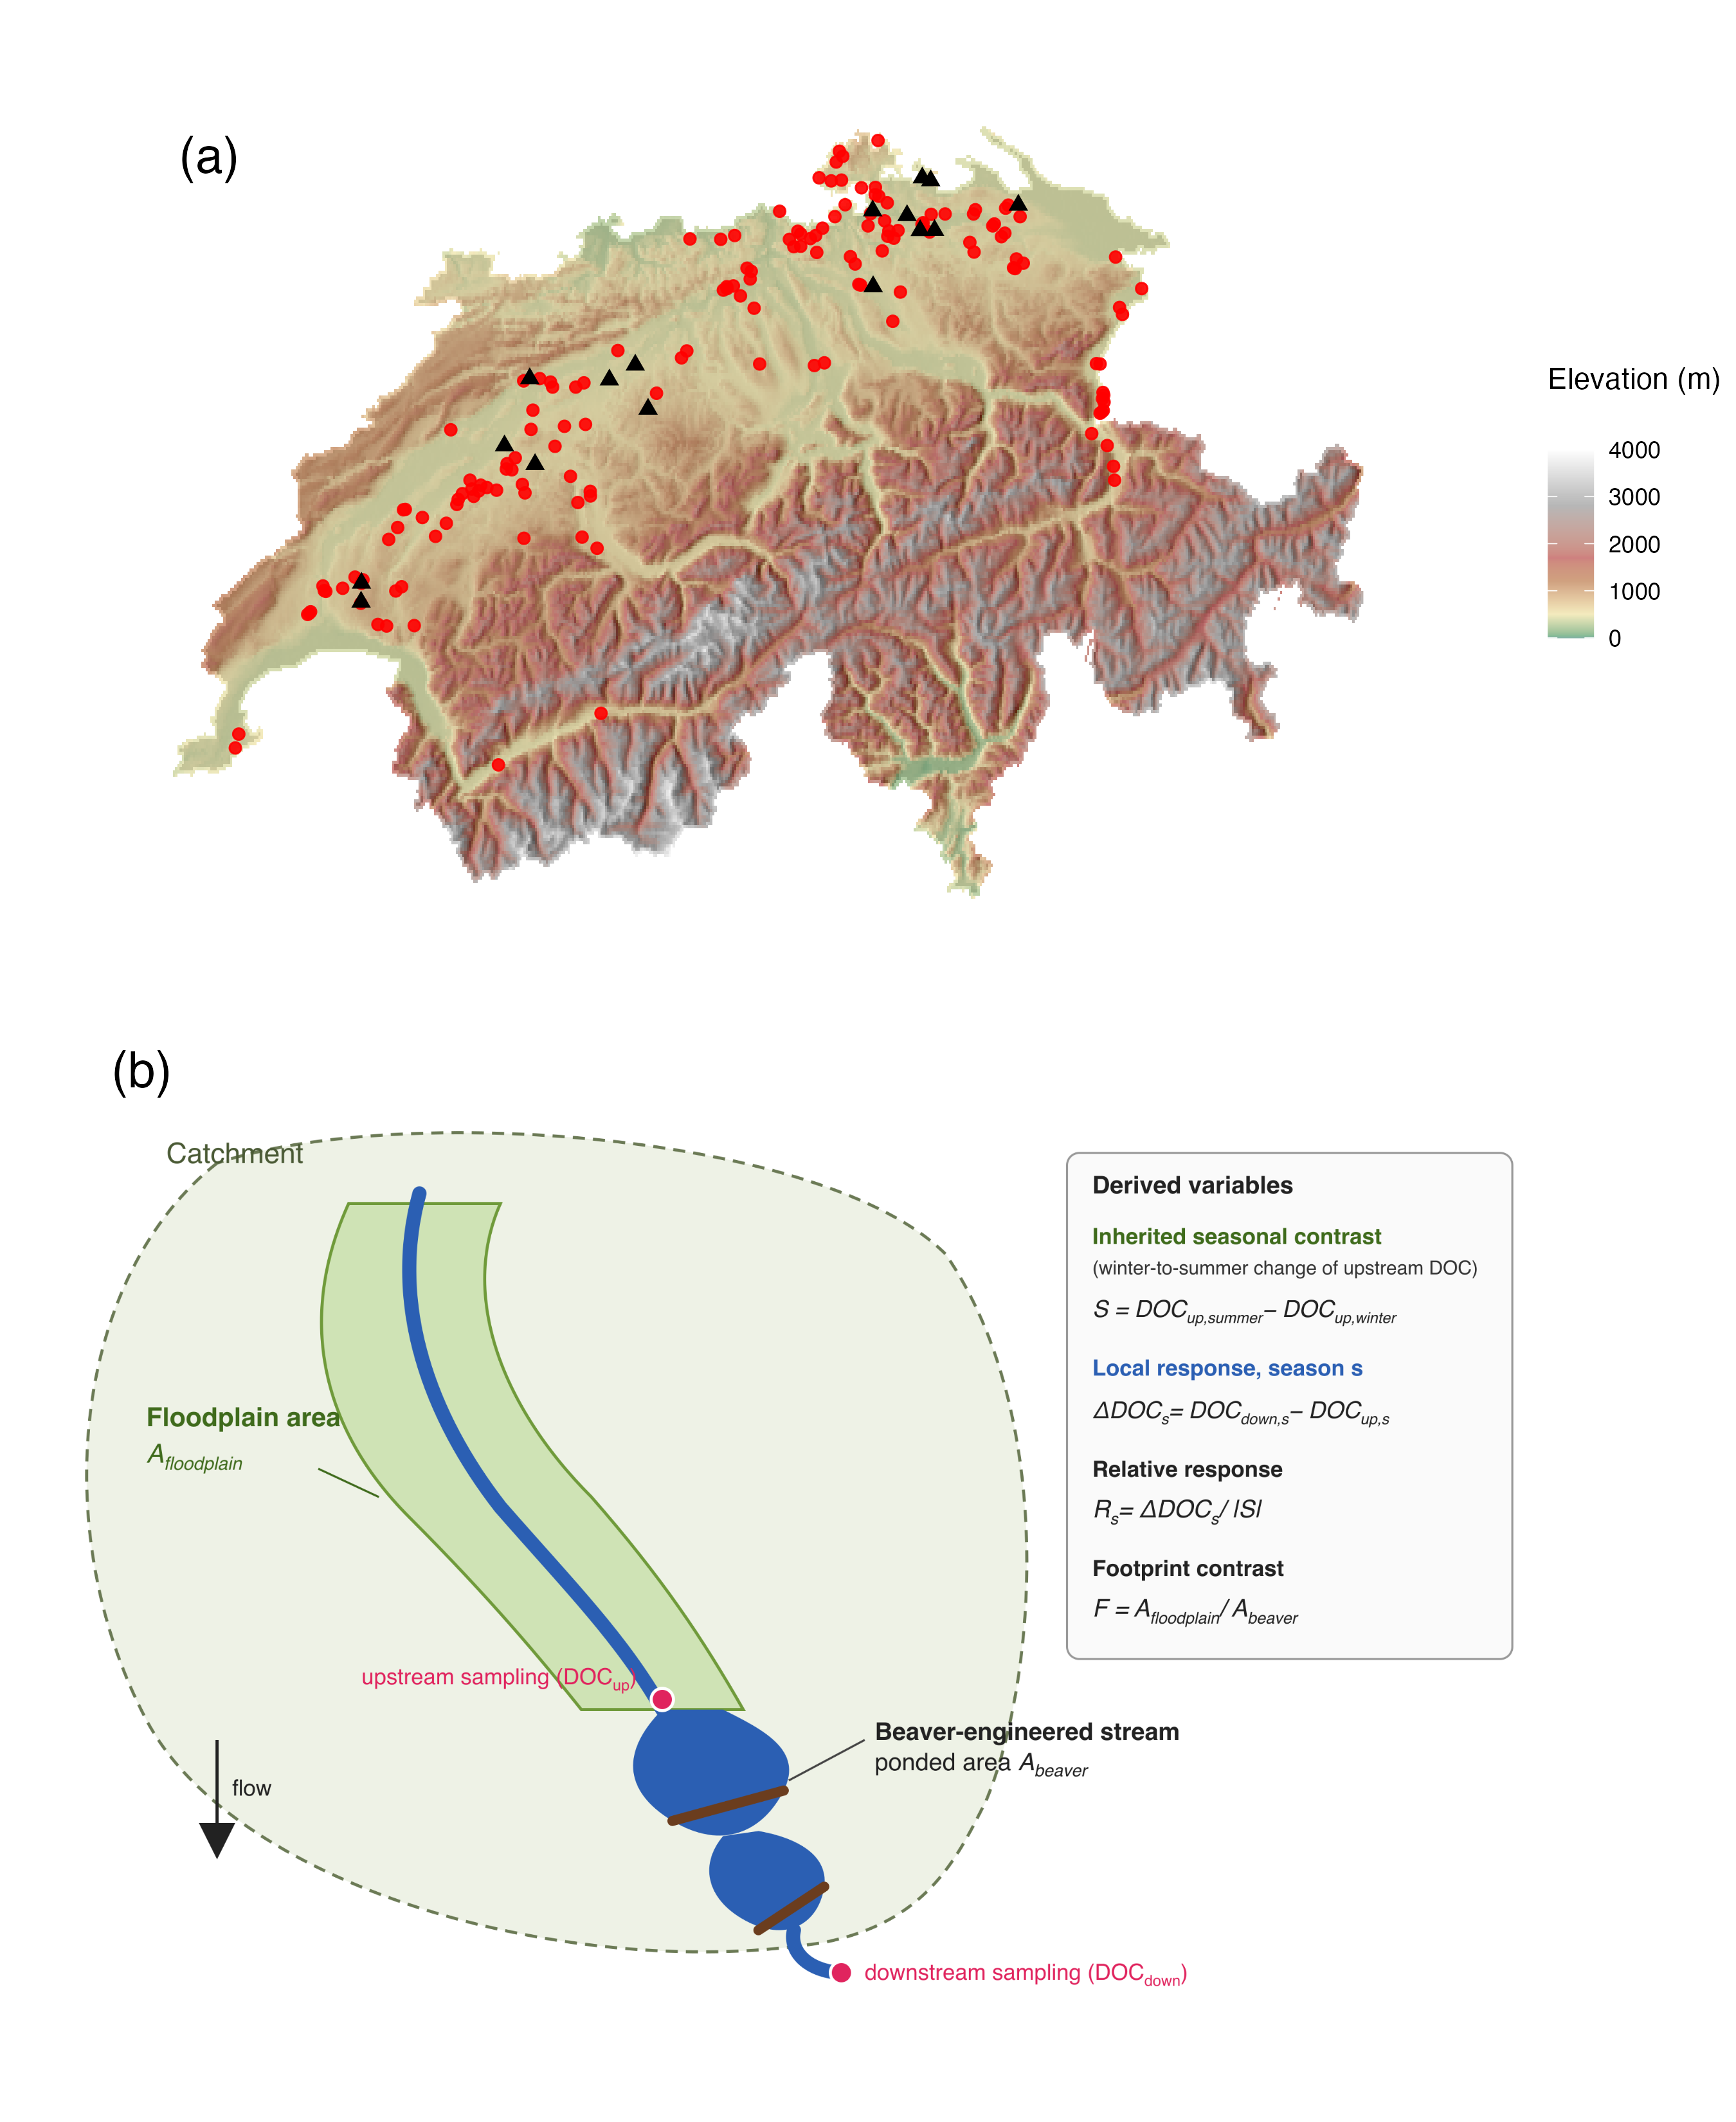
\includegraphics[width=\textwidth]{figures/media/figure1_v2.png}
\caption{a) Sampling locations across Switzerland (elevation background). Red dots (n = 158) denote streams sampled in both winter and summer; black triangles (n = 16) denote a further set of streams, sampled once in summer, where water and primary producer samples were collected. The inset shows the sampling design at each stream: water was sampled upstream of the first and downstream of the last beaver dam. b) Schematic of the derived variables. The inherited seasonal contrast \(S\) is generated over the floodplain area \(A_{floodplain}\); the local response \(\Delta DOC_s\) is measured across the beaver-engineered stream of ponded area \(A_{beaver}\); the relative response is \(R_s = \Delta DOC_s / |S|\) and the footprint contrast is \(F = A_{floodplain} / A_{beaver}\).}\label{fig:1}
\end{figure}

\subsection{Beaver engineering produces strongly variable DOC responses across streams}

Beaver-engineering did not change DOC concentrations in a consistent direction. The average \(\Delta\)DOC was 0.14 mg/L in summer (95\% Bayesian credible interval [BCI]: 0.05 ; 0.22 mg/L; P(\(\Delta\)DOC \textgreater{} 0) \textgreater{} 0.99) and 0.00 mg/L in winter (95\% BCI: -0.06 ; 0.07 mg/L), i.e., a small net DOC release in summer and none in winter, both entirely within the ROPE of \(\pm 0.5\) mg/L. Around these averages, however, individual responses were highly variable and heavy-tailed (Figure~\ref{fig:2}): for a single sampling of a beaver-engineered stream, the posterior predictive probability of a negligible \(\Delta\)DOC was 75\% in summer and 77\% in winter, of a DOC source response 16\% in summer and 12\% in winter, and of a DOC sink response 9\% in summer and 12\% in winter (95\% posterior predictive intervals: -1.9 ; 2.3 mg/L in summer, -2.1 ; 2.1 mg/L in winter). Beaver-engineered streams are therefore about as likely to increase as to decrease DOC by an ecologically relevant amount, with a slight prevalence of source responses in summer, and the heavy tails indicate that occasional large changes occur in both directions. Because \(\Delta\)DOC is bidirectional, a null average does not imply the absence of an effect: it conceals the magnitude of the change, which we quantify below relative to the seasonal contrast each stream inherits from its upstream corridor, with the relative response \(R_s\) and the seasonal gain G (third research question).

\begin{figure}[htbp]
\centering
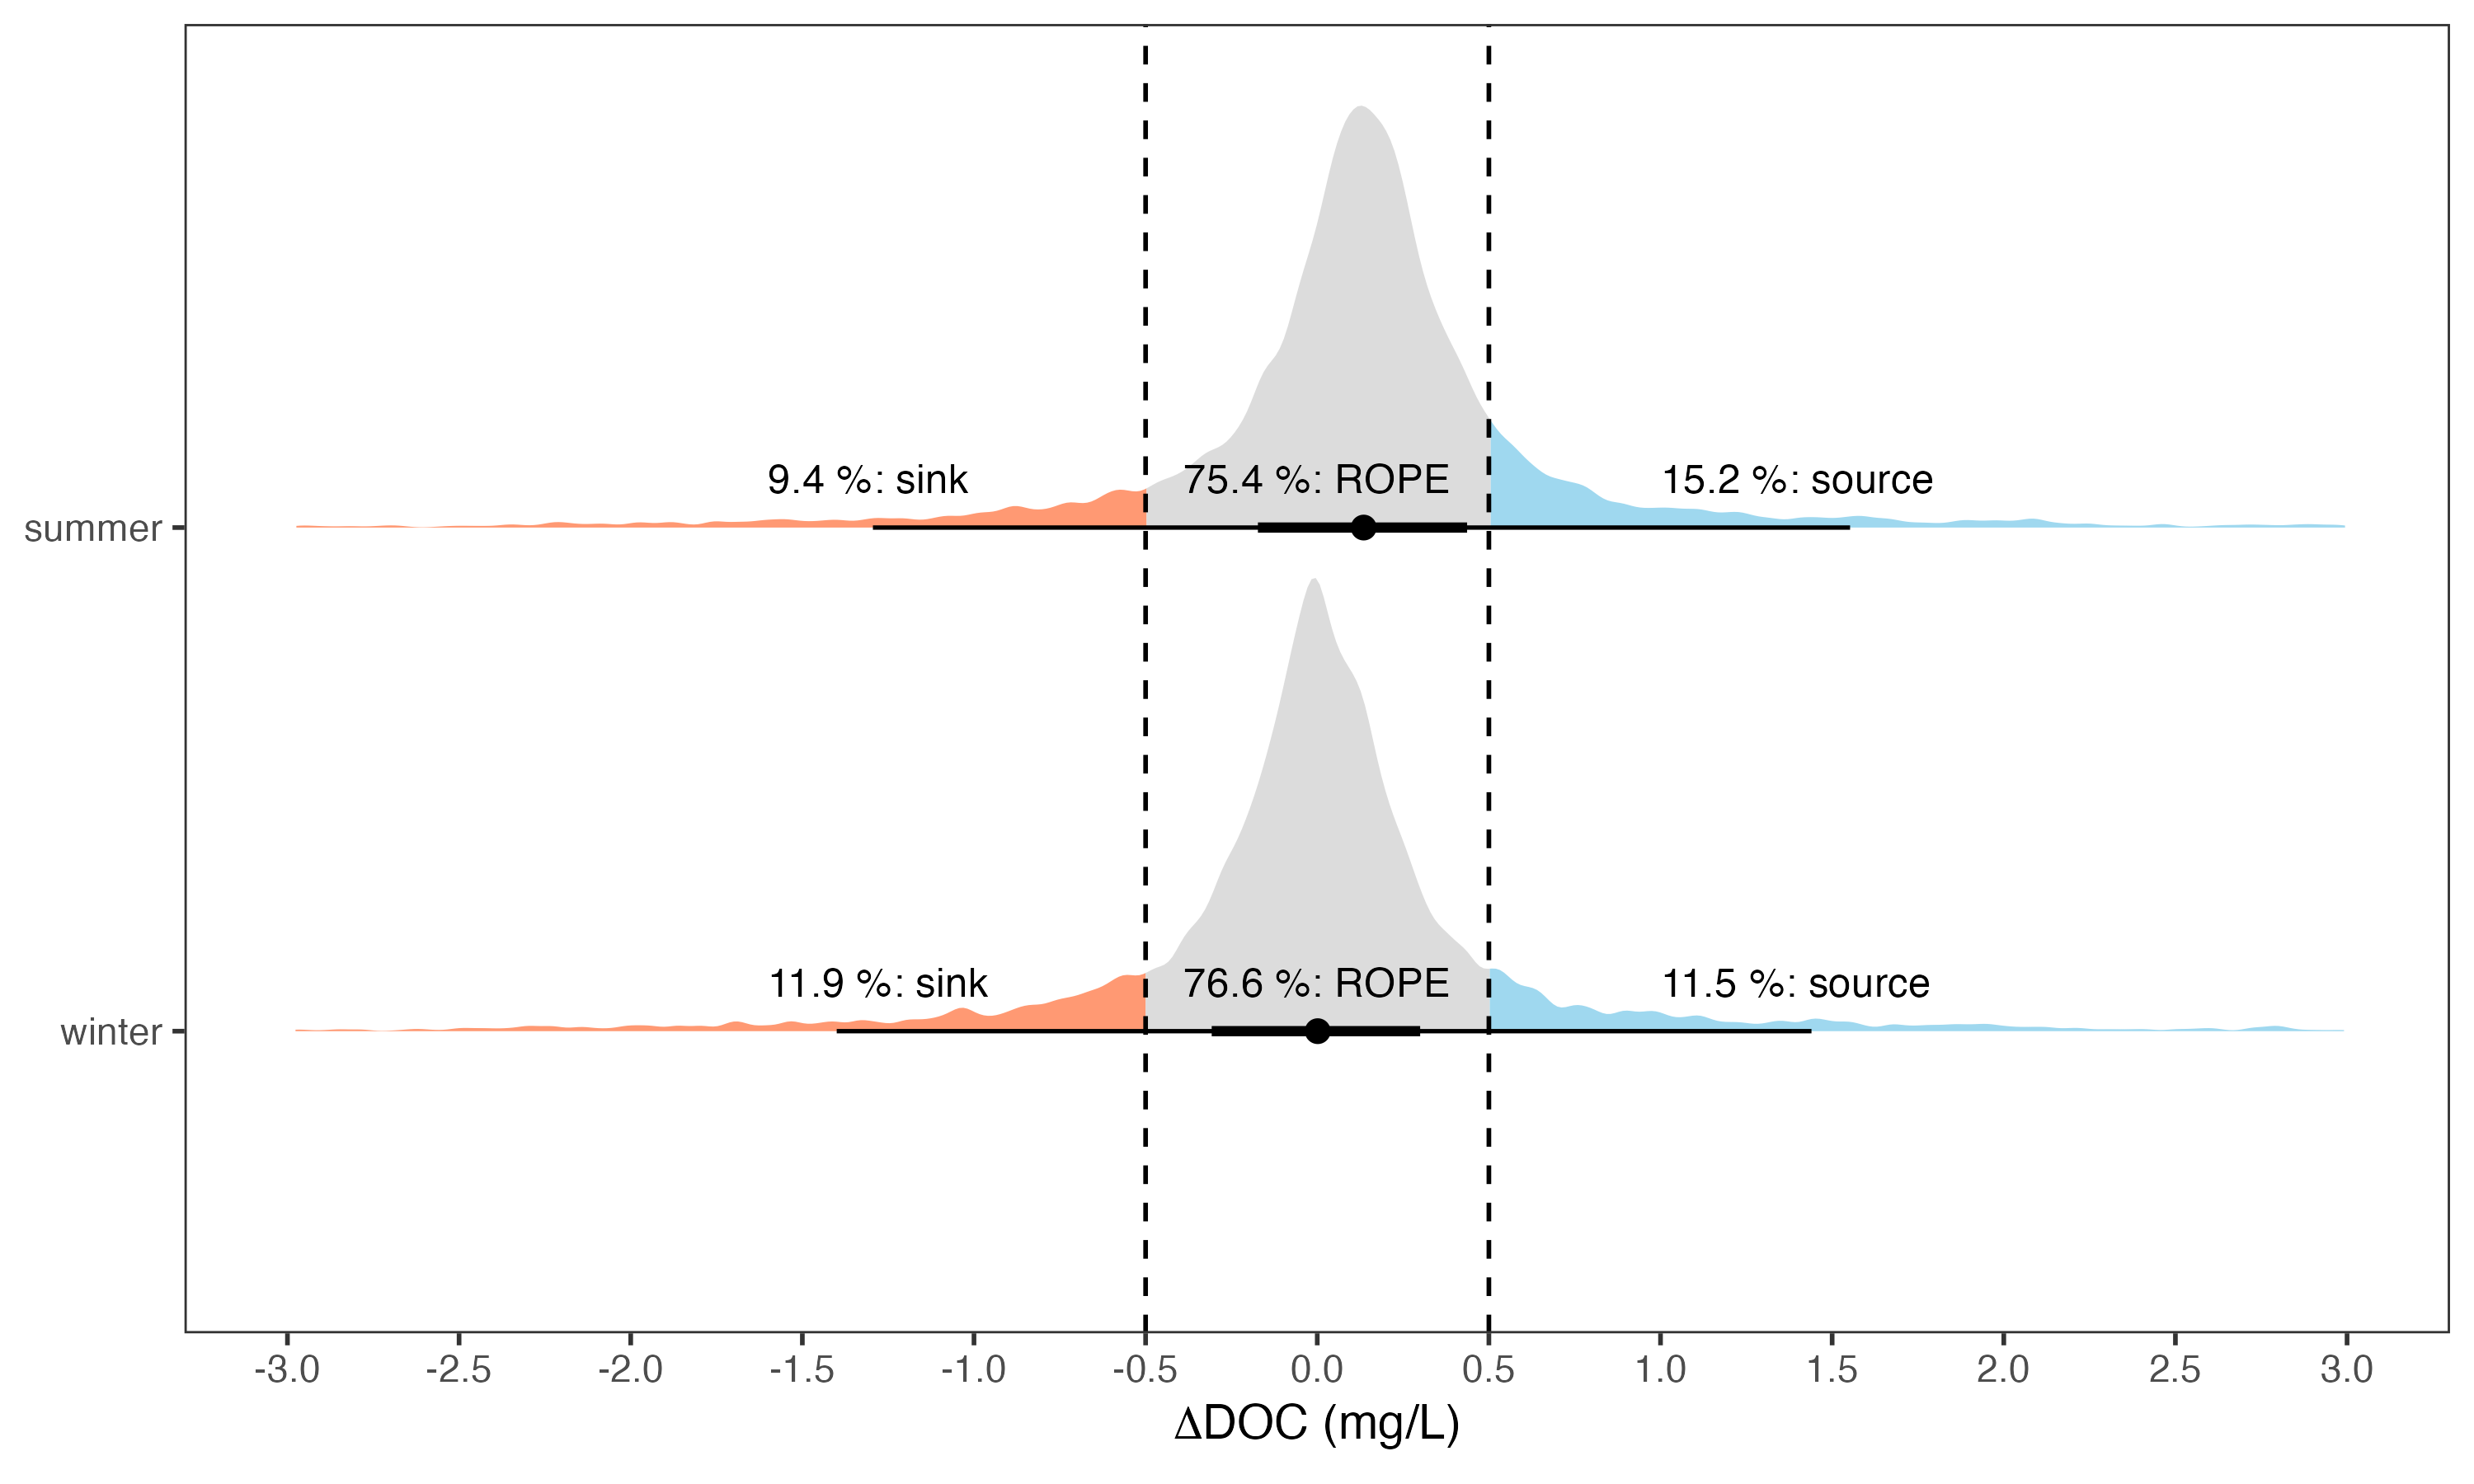
\includegraphics[width=\textwidth]{figures/media/Figure_2a.png}
\caption{Posterior predictive distribution of \(\Delta\)DOC for a single sampling of a beaver-engineered stream, in summer and winter (measurement-error model on raw upstream and downstream DOC concentrations). The orange shaded area represents the posterior predictive probability that a single sampling shows a DOC sink response; the light blue shaded area the probability of a DOC source response. The grey shaded area represents the Region Of Practical Equivalence (ROPE) and it defines an interval around zero where effects are too small to be of practical importance. The central dot indicates the median of the distribution, while the thick and thin horizontal lines represent the 66\% and 95\% intervals.}\label{fig:2}
\end{figure}

\subsection{The local response is a substantial, redistributed fraction of the inherited seasonal contrast}

\begin{figure}[htbp]
\centering
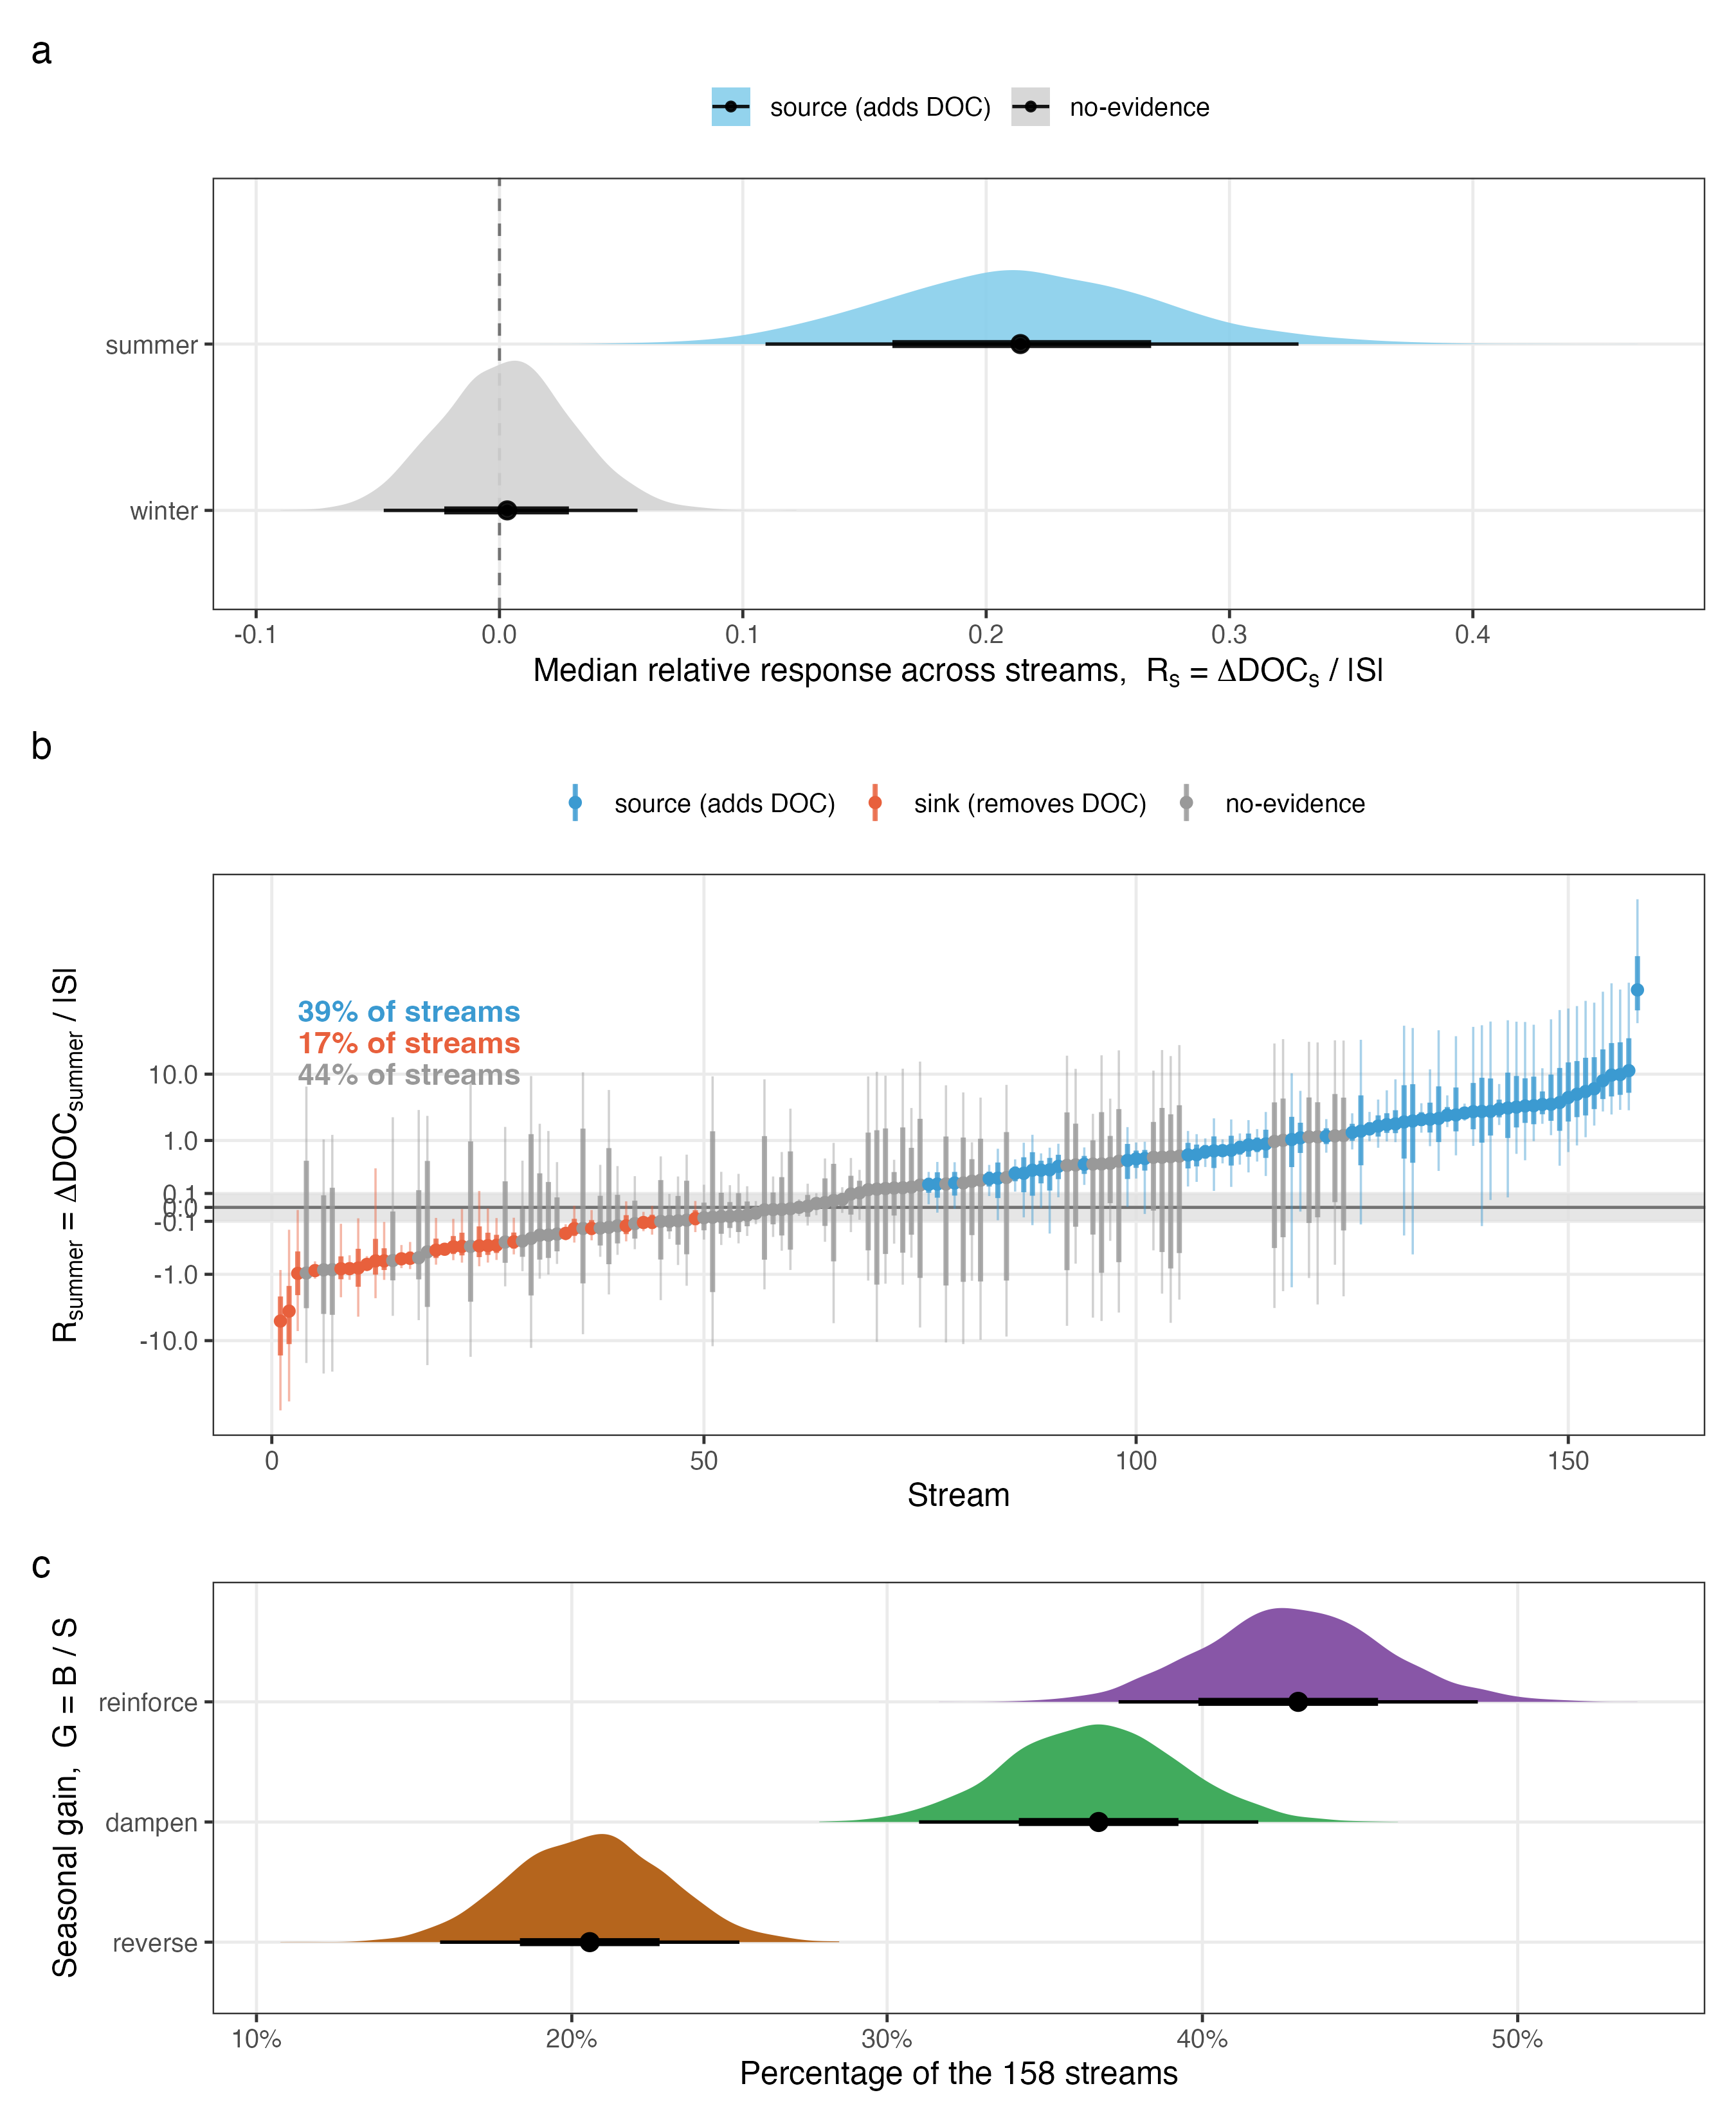
\includegraphics[width=\textwidth]{figures/media/figure3_v2.png}
\caption{a) Posterior distribution of the median relative response \(R_s = \Delta DOC_s / |S|\) across the 158 streams, in winter and summer; point: posterior median, bars: 66\% and 95\% credible intervals; dashed line: no response; skyblue: beaver-engineering adds DOC with posterior probability \textgreater{} 90\%, grey: no-evidence. b) Relative response of each stream in summer: posterior median with 66\% (thick) and 95\% (thin) credible intervals, streams ranked by their median; the grey band marks \(|R_{summer}| < 0.1\); the vertical axis is linear between -0.1 and 0.1 and logarithmic beyond. Skyblue: source (adds DOC, probability \textgreater{} 90\%), coral: sink (removes DOC, probability \textgreater{} 90\%), grey: no-evidence; percentages give the share of the 158 streams in each colour. c) Posterior share of the 158 streams whose seasonal gain \(G = B/S\) reinforces (\(G > 0\)), dampens (\(-1 < G < 0\)) or reverses (\(G < -1\)) the inherited seasonal contrast; each stream is classified on every posterior draw, so each distribution is the posterior uncertainty of the share itself; point: posterior median, bars: 66\% and 95\% credible intervals.}\label{fig:3}
\end{figure}

In summer, beaver-engineering added DOC equal to a median 21\% of the inherited seasonal contrast \(S\) across the 158 streams (95\% BCI: 11 ; 33\%), while in winter it had no net effect (Figure~\ref{fig:3}a). This average conceals substantial heterogeneity among streams (Figure~\ref{fig:3}b): in summer, 39\% of streams (62 of 158) were DOC sources and 17\% (27 of 158) were DOC sinks, with posterior probability \textgreater{} 90\%. The seasonal gain G was similarly heterogeneous (Figure~\ref{fig:3}c): 43\% of streams (95\% BCI: 37 ; 49\%) reinforced the inherited seasonal contrast, 37\% (31 ; 42\%) dampened it and 21\% (16 ; 25\%) reversed it, with a median gain across streams of G = -0.13, a mild dampening on average. Beaver-engineering therefore does not shift the seasonal contrast in one consistent direction; it redistributes it stream by stream. This local response and its redistribution of the seasonal signal occur on a small footprint: the beaver-engineered ponded area was a median 0.4\% of the floodplain area that generates the inherited seasonal contrast (footprint contrast F, median 256; Methods).

\subsection{DOC responses are associated with linked hydrological and biological pathways}

Downstream DOC was overwhelmingly set by the upstream state it inherits: the inheritance slope was 0.94 (95\% BCI: 0.89 ; 0.99 mg per mg), by far the largest path in the model (Figure~\ref{fig:4}). Around this inherited background, beaver-engineering added a local modification through the primary producers and the soil litter: phytoplankton (standardized effect +0.14) and macrophytes (+0.09) both increased downstream DOC, as did soil litter cover (+0.07). Solar radiation had a positive influence on both primary producer groups (macrophytes +0.15, phytoplankton +0.18), and water residence time had a further positive effect on phytoplankton (+0.11), itself increased weakly by the number of dams (+0.07) and decreased by channel gradient (-0.08). By contrast, we found no clear evidence that maximum dam height affected water residence time, or that water residence time directly altered downstream DOC (Figure~\ref{fig:4}). We further tested whether the incoming upstream DOC itself shapes the local response indirectly, by adding upstream DOC as a driver of the primary producers: a DOC-richer inflow was associated with more macrophytes (+0.14 per mg L\(^{-1}\), 95\% BCI: 0.00 ; 0.28) but not with more phytoplankton (-0.03, 95\% BCI: -0.15 ; 0.10); the indirect route this opens from the inflow to downstream DOC is an order of magnitude smaller than the direct inheritance and does not change the mediator effects reported above (Appendix S1: Figures S10--S11). Beaver-engineering therefore does not retain the DOC it receives from upstream; it inherits it, then adds to it through the hydrological and biological pathways it creates. This reparameterization, with downstream DOC (rather than \(\Delta\)DOC) as the outcome, is mathematically equivalent to the \(\Delta\)DOC formulation used for Q1 (Methods); a robustness check fixing the inheritance slope at 1 instead of estimating it freely left every mediator effect unchanged within its credible interval (Methods). Four alternative causal structures -- omitting the two upstream-DOC to producer links, a direct solar-radiation path to downstream DOC, and season as an unblocked confounder of the producers -- fitted no better than the reported model by leave-one-out cross-validation, and left every mediator effect unchanged (Appendix S1: Figures S10--S11). An unmeasured-confounding analysis and a prior-sensitivity check both indicate that the producer effects, based on 16 streams, are informed substantially by the literature-based priors rather than by these samplings alone (Appendix S1: Figures S12, S14), and no spatial autocorrelation remained in the model's residuals (Appendix S1: Figure S15). An alternative SCM including lateral stream--wetland connectivity as an additional driver of water residence time yielded path estimates consistent with the main model and no evidence of a connectivity effect on downstream DOC (Appendix S1: Figures S8--S9).

\begin{figure}[htbp]
\centering
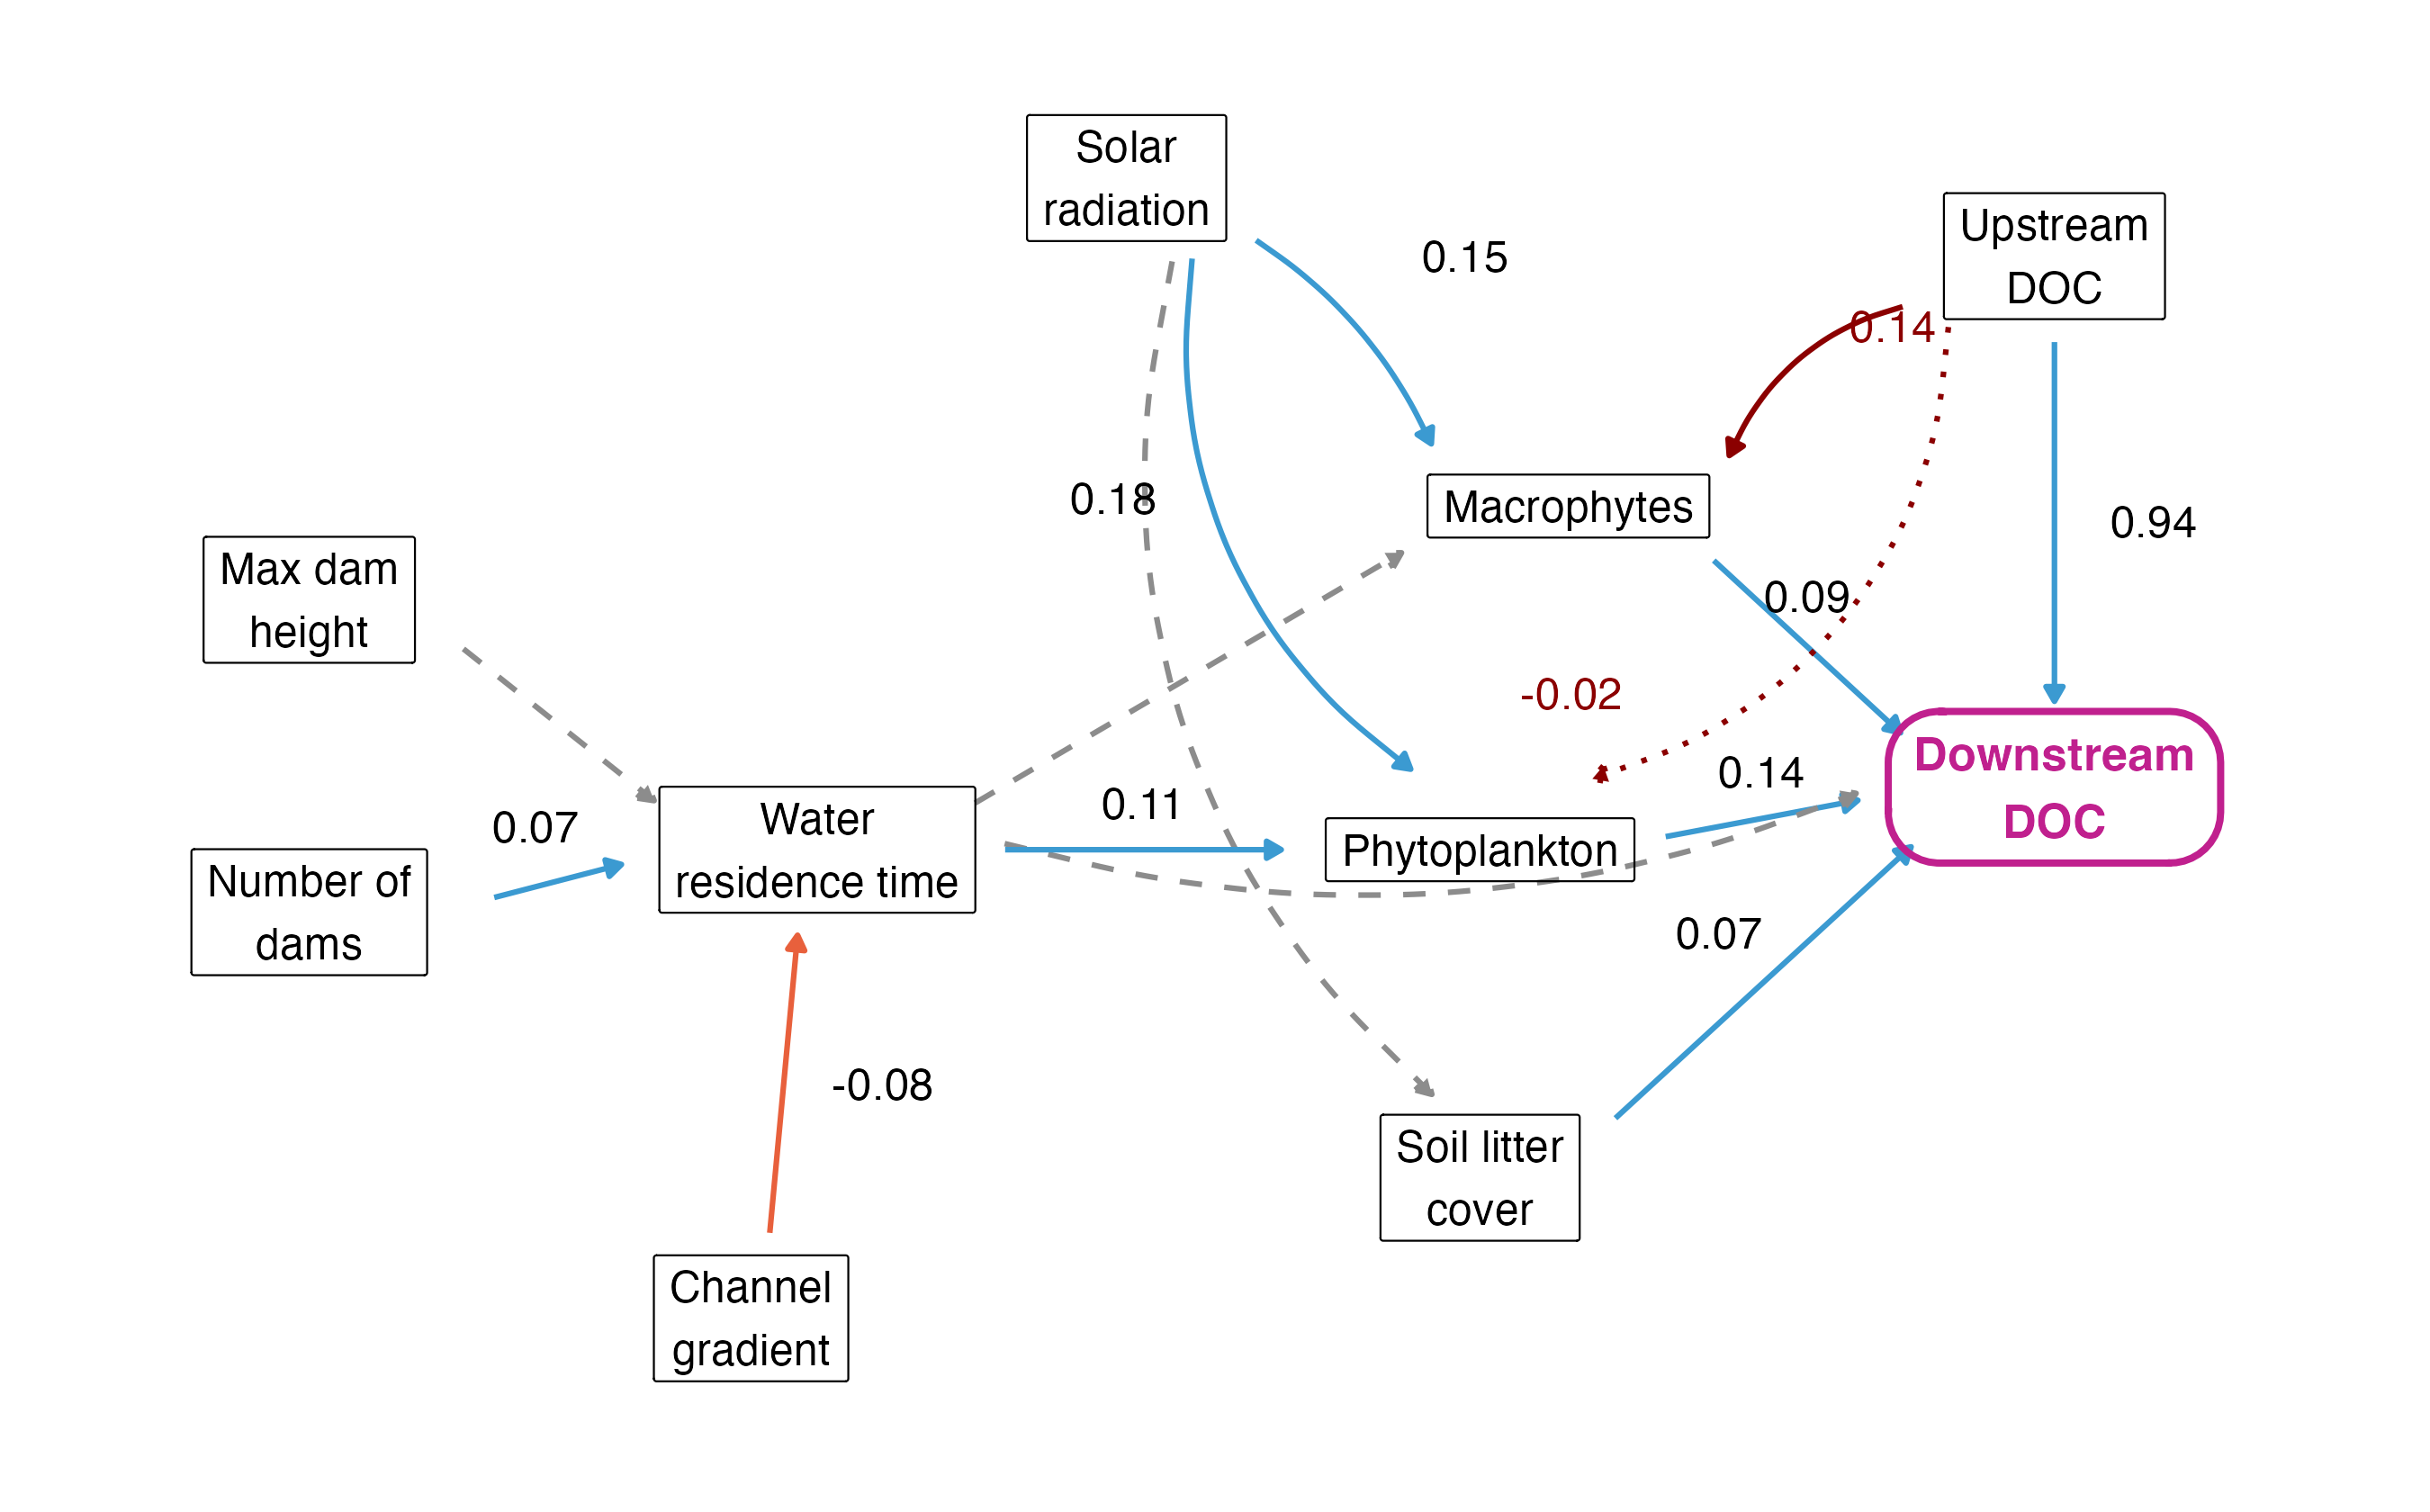
\includegraphics[width=\textwidth]{figures/media/figure4_v1.png}
\caption{Structural causal model of downstream DOC. Downstream DOC (outcome) inherits the upstream state with a freely estimated inheritance slope and is further shaped by the hydrological and biological pathways shown; solid blue edges represent \(\geq\)90\% probability evidence of a positive effect, dashed grey edges represent inconclusive evidence. Standardized posterior mean effects are shown; the upstream-DOC path is the inheritance slope in mg per mg. Dark red: the two added causal links from upstream DOC to the primary producers, tested as a sensitivity analysis (per mg L\(^{-1}\) of upstream DOC); solid meets the same \(\geq\)90\% threshold, dotted does not. Full posterior parameter distributions in Appendix S1: Figure S5.}\label{fig:4}
\end{figure}

\section{Discussion}

We found that beaver engineering does not push stream DOC in a consistent direction: across 158 streams the average change was null, yet roughly one in four samplings of a beaver-engineered reach showed an ecologically relevant DOC change, about as often a source as a sink response (with a slight prevalence of source responses in summer), and, at the level of each stream's own estimated true response, 39\% of streams resolved as clear DOC sources and 17\% as clear DOC sinks. Beaver ponds thus act as localized, intense and bidirectional DOC control points \cite{wohl2012,larsen2021}: whether a pond exports or retains DOC at a given moment is governed by local hydrology and primary producers rather than being a fixed property of the site. This context-dependence helps to reconcile the conflicting results of previous site-specific studies, which reported beaver ponds as either DOC sources or sinks \cite{larsen2021,grudzinski2022}. We also found that downstream DOC inherits the upstream state almost entirely (inheritance slope 0.94 mg per mg), and that beaver-engineering adds to that inherited background indirectly by increasing water residence time, which, in turn, enhanced aquatic primary productivity, with a further, smaller indirect route by which the incoming DOC itself feeds the macrophytes. Beaver dams are known to slow water flow and increase light penetration, creating stable habitats for phytoplankton and macrophytes \cite{johnston2017,nummi2018}. These primary producers were shown to release organic compounds and detritus and to increase DOC concentrations in dammed streams \cite{bedzki2010}. Although our estimate of the primary-producers effect on DOC was based on a relatively limited number of samples, the positive influence we detected aligns with previously documented relationships between aquatic primary productivity and DOC in lotic ecosystems \cite{allan2021}. Similar indirect effects between water flow alteration, aquatic primary productivity, and DOC were observed in other temperate and boreal streams \cite{larsen2021,grudzinski2022}. Beaver dams thus create the conditions -- ponded water, longer residence time, habitat for primary producers -- under which DOC can be rapidly produced or consumed, but whether a pond exports or retains DOC at a given moment is decided mainly by the local modification these pathways add to the inherited upstream state.

We hypothesised that the influence of beaver-engineering on DOC concentrations would be stronger in summer than in winter, owing to higher primary productivity and warmer water temperatures during the growing season. Our results supported this expectation: beaver-engineering added DOC equal to a median 21\% of the inherited seasonal contrast in summer, while in winter it had no net effect (Figure~\ref{fig:3}a). Seasonally intensified effects of beaver-engineering on DOC mirror patterns described for nutrient cycling in other aquatic ecosystems \cite{larsen2021,grudzinski2022}. The larger magnitude of change in summer likely reflects elevated primary productivity and accelerated microbial turnover \cite{mulholland1997,raza2023}, both of which are driven by increased solar radiation and warmer temperatures \cite{battin2023}. Taken together, these patterns indicate that seasonality intensifies the effects of beaver-engineering on DOC dynamics by intensifying biologically mediated C fluxes.

Beaver-mediated impacts on DOC concentrations have major implications for aquatic biogeochemistry and food-web dynamics. Elevated DOC concentrations exported during summer can enhance microbial respiration and redirect energy flow from autotrophic to heterotrophic pathways \cite{stanley2012,xenopoulos2017}. Such shifts can reduce primary production and alter consumer communities by favouring detritus-based food webs \cite{allan2021}. In winter, DOC retention and sediment C storage may support benthic microbial processes that stabilize nutrient availability and sustain overwintering invertebrates \cite{leonard2022,meyer1988}. In low-DOC ecosystems, higher beaver-induced DOC concentrations could challenge drinking-water quality, whereas in high-DOC systems, ponds may instead function as C sinks that enhance habitat complexity and energy support \cite{lemaire2022,larsen2021}.

The weak average directional response should not be interpreted as evidence that beavers had little local influence on DOC dynamics. Instead, our results reveal an important distinction between the direction and the redistribution of ecosystem change. An average of upstream--downstream DOC differences can approach zero either because little changes at individual reaches or because substantial positive and negative responses offset one another when aggregated; the pronounced variation among samplings in our study, together with the 39\% source and 17\% sink streams resolved at the level of individual reaches, is consistent with the latter interpretation. The relative response \(R_s\) and the seasonal gain G then place these same local DOC contrasts in their appropriate seasonal context: expressed relative to the inherited seasonal contrast, beaver-engineering added a median 21\% in summer, and, stream by stream, reinforced that contrast in 43\% of streams, dampened it in 37\% and reversed it in 21\%. Thus, the two results are complementary rather than contradictory. The landscape-scale average shows little coherent direction of response, whereas \(R_s\) and G show that the DOC changes that do occur are a substantial fraction of the seasonal signal each stream inherits from its corridor, and that beaver-engineering redistributes that inherited signal rather than uniformly amplifying or suppressing it. Beaver-engineering therefore increases the heterogeneity of local DOC processing without necessarily shifting landscape-average DOC in a consistent direction -- a spatiotemporal leverage exercised on a small footprint, since the beaver-engineered ponded area was a median 0.4\% of the floodplain area that generates the inherited seasonal contrast (footprint contrast F, median 256).

More broadly, these findings enhance an emerging view of river networks in which spatially discrete features can exert disproportionate control over carbon dynamics, distinguishing scale-dependent controls from patch-dependent features such as wetlands, ponds and discrete groundwater inputs that create abrupt local changes in carbon supply and processing \cite{laudon2026}. Beaver-engineering adds an important dimension to this framework because these patches are not simply inherited from the landscape: they are actively constructed and repeatedly modified by an ecosystem engineer, and their hydrological structure, biological state and therefore biogeochemical function can change as this engineering develops through time \cite{larsen2021}. Beaver-engineered reaches can therefore be understood as dynamic biogeochemical control points, whose local influence may be large even when their net directional effect is weak at broader scales. This extends the more general idea that small river-network features can have high spatial leverage \cite{wohl2025} by showing how an organism can actively create and reorganise such control points. Consistent with this relational framing, the seasonal DOC contrast that streams inherit from their corridor was spatially coherent at the regional scale, whereas the modification beaver-engineering imposed on it was spatially incoherent (Appendix S1: Figure S11): each beaver-engineered stream reinforces, dampens or reverses a regionally organised signal on its own terms, rather than beaver-engineered streams acting together as a landscape-scale control.

A null average change could also arise if the upstream--downstream difference merely reflected background spatial variability of DOC along a stream, or measurement noise, rather than a real, stream-specific response. Two observations argue against this interpretation. First, we propagated the analytical measurement error of each DOC concentration (0.2 mg L\(^{-1}\)) explicitly through the model; the 95\% posterior predictive interval of \(\Delta DOC\) (about -2 to 2 mg L\(^{-1}\)) is an order of magnitude wider, so the variability among samplings is not measurement noise. Second, once that same measurement error is accounted for in each stream's own posterior estimate of its true relative response, most streams resolve to a clear sign rather than remaining ambiguous: 39\% of streams were DOC sources and 17\% were DOC sinks with posterior probability \textgreater{} 90\%, which would not occur if the apparent responses were background noise around a single common value. We did not sample paired reaches without beaver dams, however, and a direct comparison of upstream--downstream DOC differences in un-dammed reaches of similar length remains a valuable test for future work. Likewise, we did not measure vertical (hyporheic) or lateral exchange between the channel and its floodplain, which can influence DOC independently of beaver engineering \cite{larsen2021}; our test of lateral channel--wetland connectivity (Appendix S1) found no detectable influence, but it was based on a coarse, three-level classification.

There are several further constraints on the scope of this interpretation. Our measurements describe changes in DOC concentration rather than discharge-weighted flux, so enrichment and depletion should not be interpreted as whole-system carbon sources or sinks. The mechanistic pathways were resolved from the 16 additionally characterized reaches and thus capture only part of the wider hydrogeomorphic reorganisation associated with beaver-engineering, and the two seasonal sampling periods do not resolve shorter-term event dynamics or longer-term changes as engineered reaches develop. These limitations nevertheless leave a robust central result: beaver recolonisation does not impose a uniform DOC response, but reorganises where and how strongly carbon processing occurs within river corridors.

In conclusion, by using a national-scale dataset, this study provides a comprehensive understanding of which beaver-mediated drivers influence DOC concentrations in streams. It also quantifies how the local, beaver-mediated DOC change compares with, and redistributes, the seasonal DOC contrast each stream inherits from its upstream corridor. Beaver engineering does not make streams DOC sources or DOC sinks; it creates localized control points that add to an inherited seasonal signal and reinforce, dampen or reverse it stream by stream, in a direction set by hydrology and primary producers. By identifying the environmental contexts in which these control points export or retain DOC, this work offers a predictive basis for integrating beaver presence into water-quality management and conservation planning.

\section{Methods}

\subsection{Study sites and sampling design}

We chose 180 beaver-dammed sites in Switzerland (Figure~\ref{fig:1}a). We collected water samples at upstream and downstream locations of the beaver ponds: at 158 of these streams we collected one sample in winter (December, January or February 2021/2022) and one sample in summer (June or July 2022); the remaining 22 streams were sampled once, in summer, and of these, 16 were additionally characterized for primary-producer abundance (below). We collected the upstream sample where the water was still flowing before being dammed. Since, in some cases, there was more than one dam and pond, we took the downstream sample after the last beaver dam in each sampled stream where river flow was not anymore impacted by the dam. A few streams comprised more than one separately sampled beaver-dam sequence, each with its own upstream--downstream pair; these 180 pairs are the statistical units of all models, and the paired subset of 158 (both seasons complete) is used wherever a within-stream, winter-to-summer comparison is required (direction, Q1; magnitude and seasonal modification, Q3). All sites were single-thread, low-order streams with one to several beaver dams and ponds in sequence along the channel (Figure~\ref{fig:1}a, b); none of them were extensive beaver meadows with multiple anastomosing channels and ponds at different stages of abandonment as described in North America \cite{wohl2013,larsen2021}. For each site we additionally classified the lateral connectivity between the channel and adjacent wetlands (no wetland within 50 m: 136 sites; wetland present but not connected: 11; wetland connected to the channel: 13; 22 sites unclassified) and tested its influence in an alternative structural causal model (Appendix S1). Vertical (hyporheic) and lateral exchange with the floodplain were not measured directly, which we acknowledge as a limitation when interpreting the floodplain-scale reference of the inherited seasonal contrast (below). Our dataset included a broad set of abiotic and biotic variables that are hypothesized to influence DOC concentrations in freshwater ecosystems (Figure~\ref{fig:1}; the science-based hypothesis motivating each causal path is given in Appendix S1: Table S1).

\subsection{Dissolved organic carbon net change}

In each stream, we collected water samples and filtered (0.22 \(\mu m\)) them for analysis of DOC concentration with high-temperature combustion with infrared detection of the \(CO_{2}\) produced (Shimadzu TOC-L CSH analyzer; detection limit 0.5 \(mg\mspace{6mu} C\mspace{6mu} L^{- 1}\); error measurement 0.2 \(mg\mspace{6mu} C\mspace{6mu} L^{- 1}\)). Across all sites, we calculated the net DOC concentration change (\(\Delta DOC\); as our primary response variable), by subtracting DOC concentration at downstream locations with the upstream locations.

\subsection{Beaver-engineering variables}

We defined the number of dams as the integer number of dams that we counted upstream of the downstream location. We defined the dam height (\(m\)) for each site as the maximum dam height observed upstream of the downstream location. Site persistence was defined as the number of years that beavers have inhabited the site.

\subsection{Water residence time}

We defined the water residence time (i.e., \(\tau\), seconds) using Equation~\ref{eq:wrt}:

\begin{equation}
\tau = \frac{V}{Q}
\label{eq:wrt}
\end{equation}

where \(Q\) is the stream discharge (\(m^{3}/s\)) and \(V\) is the water volume stored within the beaver's pond (\(m^{3}\)). We estimated stream water discharge using a semi-distributed hydrological catchment model (PREVAH; Precipitation-Runoff-Evapotranspiration HRU Model; \citealp{viviroli2009}). We estimated pond water volume (\(V\)) by delineating the beaver pond boundary from aerial imagery and clipping the DEM to this polygon. With the QGIS's Volume Calculation tool we then quantified the volume enclosed within the pond footprint by integrating elevation differences across all DEM cells within the polygon. We validated this method by field surveys of six different beaver ponds.

\subsection{Channel gradient}

We estimated channel gradient between upstream and downstream locations by upstream and downstream elevations from the DEM using the ``Extract values to point'' tool. We then digitized polylines that follow the swisTLM3D \cite{swisstopo2024} river line between each upstream-downstream pair and calculated their lengths (LL) with the QGIS field calculator. We computed slope as the elevation drop per horizontal distance using Equation~\ref{eq:grad}:

\begin{equation}
\text{channel gradient}\,(\%) = \frac{\text{Upstream}_{altitude} - \text{Downstream}_{altitude}}{LL} \cdot 100
\label{eq:grad}
\end{equation}

\subsection{Solar radiation}

We computed the Solar radiation (\(Wh\ m^{-2}\)) of the stream reaches with the Grass r.sun.insoltime algorithm using the \emph{qgisprocess} package in R \cite{muenchow2017}. This algorithm requires a digital surface model (DSM), a slope layer and an aspect layer. We calculated the DSM by combining a 2 m digital elevation model (DEM; \citealp{swisstopo2022}) and a 1m digital model of vegetation height (resampled to the resolution of the DEM) \cite{foen2021}. Slope and aspect were computed from the 2 m DEM using the \emph{terra} package in R \cite{hijmans2025}.

\subsection{Primary producers variables}

We sampled primary producers' abundance, namely phytoplankton, macrophyte and soil litter cover at 16 sites (Figure~\ref{fig:1}a). To estimate phytoplankton abundance, we collected 50L of water from the main beaver pond and concentrated it to a 2 L sample using a 10 μm mesh. In the laboratory, we counted and identified phytoplankton with a dual-magnification dark-field imaging microscope that captured all particles in the size range between \textasciitilde10 μm and \textasciitilde1 cm using a 5.0× magnification objective. We estimated macrophyte abundance by counting each individual plant detected in the beaver ponds. We estimated soil litter percentage cover in a 1x5 m plot located at 0.5 m distance from the edge of the beaver pond in each site. We defined all dead plant material, such as leaves, but also twigs \textless7cm circumference, as soil litter.

\subsection{Statistical analyses}

\subsubsection{Direction of the beaver-mediated DOC change (first research question)}

To estimate the direction of the beaver-mediated DOC change we modelled the raw upstream and downstream DOC concentrations rather than their pre-computed difference, so that the analytical measurement error of each concentration (0.2 mg L\(^{-1}\)) is propagated exactly to \(\Delta DOC\). We fitted a Bayesian hierarchical measurement-error model in which the observed concentration of each sample is a noisy measurement of a latent true concentration (\texttt{mi(0.2)} in \emph{brms}), and the latent concentrations follow a Student-\(t\) distribution (to accommodate the heavy-tailed distribution of DOC) whose mean is a season \(\times\) location (upstream/downstream) factorial, with random intercepts for stream and for stream \(\times\) season that pair the upstream and downstream samples of the same stream and sampling occasion \cite{gelman2013}. The average \(\Delta DOC\) of each season is derived from the posterior as the difference between the downstream and upstream season means, and the posterior predictive distribution of \(\Delta DOC\) for a single sampling of a stream as that difference plus the difference of two residual draws. We considered a net change in DOC larger than \(0.5\ mg/L\) as ecologically relevant: when \(\Delta DOC > 0.5\ mg/L\), the pond is a DOC source within the ecosystem; when \(\Delta DOC < - 0.5\ mg/L\), the pond is a DOC sink. We applied the Bayesian Region of Practical Equivalence (ROPE) to values between \(- 0.5\ and\ 0.5\ mg/L\); the ROPE defines an interval around zero where effects are too small to be of importance \cite{pan2025}. This \(\pm 0.5\ mg/L\) threshold is justified because changes of this magnitude are near levels at which DOC concentrations begin to affect light penetration, nutrient dynamics, and the balance between autotrophy and heterotrophy in freshwater ecosystems \cite{thrane2014,seekell2015}. We applied the ROPE (i) to the posterior of the seasonal average \(\Delta DOC\) and (ii) to the posterior predictive distribution of \(\Delta DOC\) for a single sampling (Figure~\ref{fig:2}): the shares of the latter below, within and above the ROPE are the posterior predictive probabilities that one sampling of a beaver-engineered stream shows a sink, a negligible or a source response. These probabilities describe the variability of individual responses and are not percentages of streams; with two samplings per stream, stream-specific \(\Delta DOC\) values cannot be resolved (Appendix S1: Figure S6).

\subsubsection{Drivers of the beaver-mediated DOC change: structural causal model (second research question)}

To answer the second research question, we used a two-step analytical approach combining causal modeling and Bayesian inference to integrate prior knowledge and account for uncertainty in our parameter estimates. First we described the set of possible data-generating processes that we hypothesized to be causing \(\Delta DOC\) variation (i.e., Structural Causal Model, SCM; the hypothesized DAG is shown in Figure~\ref{fig:4} and, with its thirteen causal paths numbered, in Appendix S1: Figure S1; each numbered path corresponds to one science-based hypothesis motivated in Appendix S1: Table S1) \cite{arif2023}. As a structural sensitivity analysis, we additionally tested two further causal links from upstream DOC to the primary producers, alongside a direct solar-radiation path to downstream DOC and season as an unblocked confounder of the producers (Appendix S1: Figures S10--S14). Second, we proceeded to infer the relationships between variables using a multivariate linear model within a Bayesian framework. A DAG makes the causal assumptions of an analysis explicit, and the identification of causal effects is conditional on those assumptions \cite{pearl2009,arif2023}. Because different DAGs encode different hypotheses on how the system works, it is recommended to specify and test alternative DAGs and to report their estimates transparently, so that the robustness of the conclusions to the assumed causal structure can be assessed \cite{tennant2021,laubach2021}. We therefore also tested an alternative, extended SCM in which the lateral connectivity between the stream and adjacent wetlands influences water residence time, and hence \(\Delta DOC\) (Appendix S1: Figures S8--S9). The full model specification is given below (Equation~\ref{eq:scm}); the tested hypotheses for each causal path, the priors, residuals and posterior predictive checks are reported in Appendix S1 (Figures S2--S4). In the SCM, \(\Delta DOC\) enters as the outcome with its propagated measurement error (Equations~\ref{eq:err}--\ref{eq:scm}).

In this study we used the structural causal model (SCM) framework to answer the research questions (\emph{sensu} \citealp{arif2023}). The SCM can be considered as a directed acyclic graph (DAG) with nodes and edges. The nodes indicate the relevant variables of the ecosystem and the edges indicate direct causal influences. The edges are acyclic because a cause is not at the same time an effect. We fitted the SCM with the Bayesian framework to accommodate the uncertainty inherent in ecological data and to incorporate prior distributions based on previous research and expert opinion \cite{gelman2013}.

We specified the SCM model as a system of linear equations, where each equation represents the relationship between a response variable and its predictors. We statistically defined the full Bayesian SCM as in Equation~\ref{eq:scm}.

Given that the error in both the downstream and upstream DOC measurements was 0.2 \(mg\mspace{6mu} C\mspace{6mu} L^{- 1}\), we estimated the error of \(\Delta DOC\) (i.e., \(E\)) by error propagation using Equation~\ref{eq:err}:

\begin{equation}
E = \sqrt{0.2^{2} + 0.2^{2}} = \sqrt{0.08} \approx 0.283\ mg\ L^{-1}
\label{eq:err}
\end{equation}

Specifically, we treated the measurement error as missing data and imputed it using a normal distribution with a mean of 0 and a standard deviation of 0.283 mg/L. The overall model comprised a measurement model and an outcome multivariate model. First, we accounted for observational uncertainty by specifying a measurement model that links the observed \(\Delta DOC_{i}^{obs/imputed}\)~to a latent (true) DOC change, \(\Delta DOC_{i}^{true}\):

\begin{equation}
\begin{aligned}
\textbf{Measurement model:} \quad
\Delta \text{DOC}_i^{\text{obs}} &\sim \mathcal{N}(\Delta \text{DOC}_i, 0.283^2) \\
\text{DOC}_{\text{upstream},i}^{\text{obs}} &\sim \mathcal{N}(\text{DOC}_{\text{upstream},i}, 0.2^2) \\[1em]
\textbf{Outcome multivariate model:} \quad
\Delta \text{DOC}_i &\sim \text{Student-}t(\nu, \mu_i, \sigma_{\Delta \text{DOC}}) \\
\mu_i &= \beta_1 \cdot \text{DOC}_{\text{upstream}, i} \\
&\quad + \beta_2 \cdot \text{Macrophytes}_i \\
&\quad + \beta_3 \cdot \text{Phytoplankton}_i \\
&\quad + \beta_4 \cdot \text{Litter Cover}_i \\
&\quad + \beta_5 \cdot \text{WRT}_i \\[1em]
\textbf{Predictors multivariate model:} \quad
\text{Macrophytes}_i &\sim f(\text{solar radiation}_i, \text{WRT}_i, \text{DOC}_{\text{upstream},i}, \dots) \\
\text{Phytoplankton}_i &\sim f(\text{Macrophytes}_i, \text{WRT}_i, \text{DOC}_{\text{upstream},i}) \\
\text{Litter Cover}_i &\sim f(\text{solar radiation}_i) \\
\text{WRT}_i &\sim f(\text{DamHeight}_i, \text{NDams}_i, \dots) \\
&\ \ \vdots \\[1em]
\textbf{Priors:} \quad
\alpha_{\text{summer}} &\sim \mathcal{N}(0, 10) \\
\alpha_{\text{winter}} &\sim \mathcal{N}(0, 7.5) \\
\beta_2, \beta_3, \beta_4, \beta_5 &\sim \mathcal{N}(0.05, 0.1) \\
\beta_6 &\sim \mathcal{N}(0, 0.2) \\
&\ \ \vdots \\
\sigma_{\Delta \text{DOC}} &\sim \text{Student-}t(3, 0, 2.5) \\
\sigma_{\text{upstream}} &\sim \mathcal{N}(0, 0.5) \\
\nu &\sim \text{Gamma}(2, 0.1)
\end{aligned}
\label{eq:scm}
\end{equation}

We used the mi() function from the R package \emph{brms} (version 2.23) to account for the measurement error of 0.283 mg/L on the response variable \(\Delta DOC\). We imputed missing data during model fitting by treating them as additional parameters. We ensured that missing data in both response and predictor variables were modeled rather than excluded by using the mi() function. This function treats missing values as additional parameters and estimates them jointly with the model.

We generated 20,000 (four chains run for 10,000 iterations discarding the first 3000 as burn-in) Markov chain Monte Carlo (MCMC) samples from the posterior distribution. We visually assessed if the SCM was a reasonably good description of the data by posterior predictive check and residuals (Appendix S1: Figures S3 and S4). All MCMC chains indicated convergence through falling within the threshold (i.e., R-hat \textless{} 1.05) specified by Gelman and Rubin \cite{gelman1992}.

For Figure~\ref{fig:4} we report the same SCM in a reparameterization with downstream DOC (rather than \(\Delta DOC\)) as the outcome: upstream DOC enters as a latent true concentration, carrying its own 0.2 mg L\(^{-1}\) instrument error, as the inherited incoming state with a freely estimated inheritance slope (prior Normal(1, 0.3)), and \(\Delta DOC\) is derived from the posterior afterwards as the difference between the downstream and upstream estimates, so upstream DOC is never simultaneously a predictor and part of the response. This reparameterization is mathematically equivalent to Equation~\ref{eq:scm}: every mediator effect agreed with the \(\Delta DOC\)-outcome model to the second decimal, and the upstream-DOC path is re-read as an inheritance slope (0.94, 95\% BCI: 0.89 ; 0.99 mg per mg) instead of a standardized effect on \(\Delta DOC\). As a robustness check, we refitted this model with the inheritance slope fixed at 1 (prior Normal(1, 0.001)) instead of estimated freely; every mediator effect, and both of the upstream-to-producer links below, remained within its credible interval, confirming that the mediator pathways do not depend on how the inheritance slope is handled. We further extended both parameterizations with two causal links from upstream DOC to the primary producers (macrophytes, phytoplankton), to test whether the incoming DOC concentration also shapes the local response indirectly through the producers, in addition to setting the inherited background directly (Figure~\ref{fig:4}); this extended structure, and three further alternative causal structures, are compared by leave-one-out cross-validation in Appendix S1 (Figures S10--S11).

If posterior parameter distributions had more than 90\% probability mass on either side of zero (\(P(\beta > 0)\) or \(P(\beta < 0)\)), then we assumed that there was statistical evidence for the positive or negative effect of the predictor on the response variable.

We did all the data cleaning and statistical analysis within the R environment (version 4.6.1). We conducted data cleaning with the tidyverse (version 2.0.0) package and created figures using ggplot2 (version 4.0.3). We used the R packages \emph{brms} (version 2.23), tidybayes (version 3.0.7), and bayesplot (version 1.15.0), with the CmdStan backend via cmdstanr (version 0.9.0), for Bayesian inference.

\subsection{Relative response and seasonal gain}

To answer the third research question we defined a small set of quantities derived from the upstream and downstream DOC concentrations of each stream (Figure~\ref{fig:1}b). The inherited seasonal contrast (\(S\); \(mg\ L^{-1}\)) is the winter-to-summer change of upstream DOC, i.e. what the upstream corridor delivers to the stream irrespective of beaver-engineering (Equation~\ref{eq:S}):

\begin{equation}
S = DOC_{upstream}^{summer} - DOC_{upstream}^{winter}
\label{eq:S}
\end{equation}

The local response in season \(s\) (\(\Delta DOC_s\); \(mg\ L^{-1}\)) is the change in DOC that beaver-engineering produces across the stream (Equation~\ref{eq:ddocs}):

\begin{equation}
\Delta DOC_s = DOC_{down,s} - DOC_{up,s}
\label{eq:ddocs}
\end{equation}

The relative response (\(R_s\); dimensionless) expresses the local response as a fraction of the inherited seasonal contrast, so that \(R_s > 0\) indicates beaver-engineering adds DOC and \(R_s < 0\) indicates it removes DOC, relative to the magnitude of the seasonal signal the stream inherits (Equation~\ref{eq:Rs}):

\begin{equation}
R_s = \frac{\Delta DOC_s}{|S|}
\label{eq:Rs}
\end{equation}

The beaver seasonal modification (\(B\); \(mg\ L^{-1}\)) is how much beaver-engineering changes the winter-to-summer DOC contrast itself (Equation~\ref{eq:B}):

\begin{equation}
B = \Delta DOC_{summer} - \Delta DOC_{winter}
\label{eq:B}
\end{equation}

and the seasonal gain (\(G\); dimensionless) expresses \(B\) as a fraction of \(S\), distinguishing whether beaver-engineering reinforces (\(G > 0\)), dampens (\(-1 < G < 0\)) or reverses (\(G < -1\)) the inherited seasonal contrast (Equation~\ref{eq:G}):

\begin{equation}
G = \frac{B}{S}
\label{eq:G}
\end{equation}

Because \(S\) can be small for individual streams, forming \(R_s\) and \(G\) from raw concentrations would let small denominators dominate the ratio. We therefore computed all four quantities from the posterior of a Bayesian hierarchical measurement-error model fitted separately to each of the four measured concentrations (upstream winter, downstream winter, upstream summer, downstream summer): each concentration was modelled on the log scale with its known 0.2 mg L\(^{-1}\) instrument error and a random intercept per stream, so that each stream's estimated true concentration -- not the raw reading -- was used to compute \(S\), \(\Delta DOC_s\), \(R_s\), \(B\) and \(G\), and the full posterior uncertainty of each derived quantity was carried through from 4000 posterior draws per stream. \(R_s\) and \(G\) were classified per stream (source/sink for \(R_s\); reinforce/dampen/reverse for \(G\)) when the posterior probability of that classification exceeded 90\%; population-level shares by classification (Figure~\ref{fig:3}b, c) were computed by classifying every stream on every posterior draw and taking the proportion of streams in each class per draw, so that the reported share itself carries a posterior distribution rather than being a single count.

Finally, we defined the footprint contrast (\(F\); dimensionless) as the ratio of the floodplain area that generates \(S\) to the ponded beaver-engineered area (Equation~\ref{eq:F}), to express how small the engineered footprint is relative to the corridor over which the inherited seasonal contrast is generated:

\begin{equation}
F = \frac{A_{floodplain}}{A_{beaver}}
\label{eq:F}
\end{equation}

The delineation of the catchment and floodplain area of each site is described below.

\subsubsection{Definition of catchment and floodplain area}

We delineated the catchment area by automatically assigning pour points to stream outlets at each site and entering these, along with a D8 pointer raster based on a 25 m DEM \cite{swisstopo2004} into the \emph{Watershed} algorithm in Whitebox \cite{lindsay2016} executed using the \emph{Whitebox} package in R \cite{wu2022}. We calculated the floodplain area of each site using a custom-made function in R based on the elevation differential of the local terrain and the nearest channel, adapted from a method developed by Clubb et al. \cite{clubb2017}.

\backmatter

\bmhead{Data and code availability}

We confirm that all codes for data processing, including the processed data, main analyses, and supplemental analyses, are available on the GitHub repository \url{https://github.com/leomarameo7/beavers_DOC}.

\bmhead{Acknowledgments}

We thank all the volunteers and Master students who collected water samples and ecological data. We thank Marta Reyes, Denise Freudemann and the central laboratory of the Swiss Federal Institute for Aquatic Ecology (Eawag) for subsequent laboratory analysis of DOC concentrations. We thank the ETH Board for financing the study as part of the Blue-\-Green Initiative. Finally, we would like to thank the Federal Office for the Environment FOEN for the financial support of the research project, which was the basis for the selection of beaver territories for this study.

\bmhead{Author contributions}
 conceptualization: Leonardo Capitani, Matthew Dennis, Lukas Hallberg, Annegret Larsen, Joshua R. Larsen, Valentin Moser, Francesco Pomati, Anita C. Risch; data collection and curation: Christof Angst, Kaspar Berger, Steffen Boch, Matthew Dennis, Annegret Larsen, Joshua Larsen, Silvan Minnig, Valentin Moser, Massimiliano Zappa, Francesco Pomati, Anita C. Risch; formal and statistical analysis: Leonardo Capitani; visualization: Leonardo Capitani; writing---original draft: Leonardo Capitani; writing---review and editing: all authors.

\bmhead{Funding information}

The study was funded by ETH Board through the Blue-Green Biodiversity (BGB) Initiative (2021--2024) and by the Swiss Federal Office for the Environment (FOEN).

\bmhead{Conflict of interest statement}

We declare no conflict of interest.

\bmhead{Supplementary information}
Appendix S1 (Table S1--S2, Figures S1--S15) is provided as a separate file: \texttt{supplementary/appendix\_S1.pdf}.

\bibliography{references}

\end{document}
